\subsection{Carrucole} \label{carrucole}

\subsubsection{Corpi appesi a fili}

\begin{enumerate} % corpi appesi a fili

\item % corpi appesi a fili
\label{car_x_01}
Un corpo di massa $mc = 7 kg$ è appeso al soffitto di una stanza mediante un filo di massa
$mf = 50 g$ ed è in quiete.


\begin{enumerate}
\item Trovare la forza che il corpo esercita sul filo
\item Trovare la forza che il soffitto esercita sul filo
\end{enumerate}

Soluzione a pagina \pageref{car_s_01}


\end{enumerate} % corpi appesi a fili



\subsubsection{Due Carrucole e una forza}

\begin{figure}[h]
\centering
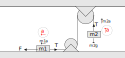
\includegraphics[width=0.8\textwidth]{carrucole.pdf}
\end{figure}

\begin{itemize}
\item $m_1=50$
\item $m_2=80$
\item $F=1N$
\end{itemize}

L'accelerazione $a$ è l'incognita che dobbiamo trovare.

Per ognuna delle due masse si genera una forza di inerzia che si oppone in senso inverso alla causa del moto.

Le forze di inerzia sono $m_1a$ e $m_{2}a$, in senso contrario all'accelerazione.

Nota bene: Durante l'impostazione del problema non è ancora chiaro quale sia il senso del moto dei vari pesi.

Non so se un peso si muove in un modo o nell'altro.

Quindi all'accelerazione incognita (in rosso) è stato assegnato un senso arbitrario, giusto per capire quale forza si oppone a quale altra e quindi dove mettere i $+$ e i $-$.

Alla fine otterrò un numero che potrà essere negativo o positivo; questo sarà il modulo della forza.

Le forze in ognuno dei due sistemi costituito da peso e corda si equivalgono; vuol dire che la loro somma è zero.

Nel primo peso la somma di queste forze deve essere zero:

\begin{enumerate}
\item $F$: la forza applicata alla prima massa
\item $m_1a$: la forza applicata dall'accelerazione risultante
\item $-T$ la tensione della corda, negativa perché tira in senso opposto
\end{enumerate}

Posso quindi scrivere che:
\setcounter{equation}{0}

\begin{equation}
\left\{
\begin{array}{ll}
F + m_1a -T = 0\\
m_2g -T - m_2a =0
\end{array}
\right.
\end{equation}

Quindi

\begin{equation}
\Rightarrow
\left\{
\begin{array}{ll}
T - F = m_1a\\
m_2g -T = m_2a
\end{array}
\right.
\end{equation}

Dalla prima ricavo $T$:


\begin{equation}
T = F + m_1a
\end{equation}

Sostituisco nella seconda

\begin{equation}
m_2g -F - m_1a = m_2a
\end{equation}

Sposto $m_1a$ a destra

\begin{equation}
m_2g -F = m_1a + m_2a
\end{equation}

Raccolgo $a$:

\begin{equation}
m_2g -F = a(m_1 + m_2)
\end{equation}

Ed ecco $a$:

\begin{equation}
a=\frac{
m_2g -F
}{
m_1 + m_2
}
\end{equation}

Ora posso sostituire i valori iniziali:

\begin{equation}
a=\frac{ m_2g -F }{ m_1 + m_2 } =  \\
\frac{80-1}{80+50} = \\
\frac{79}{130} = \\
.53846153846153846153
\end{equation}


\begin{minipage}{\textwidth}

\subsubsection{Una Carrucola e tre pesi}

\begin{figure}[H]
\centering
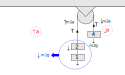
\includegraphics[width=0.8\textwidth]{carrucole.2}
\end{figure}

\begin{itemize}
\item $m_1=2 kg$
\item $m_2=4 kg$
\item $m_3=1 kg$
\end{itemize}

\end{minipage}

\begin{enumerate}
\item \textbf{Find the acceleration of the 4 kg block.}

Per quanto riguarda $a$, i pesi da 1 3 possono essere considerati come una unica massa che chiameremo $m_1$.

La forza di inerzia corrispondente è $m_1g$.

Notare il senso delle frecce nel disegno: indicano il segno delle varie forze.

per esempio $m_1g$ è diretta in basso; all'inizio abbiamo deciso arbitrariamente che $a$ vada nella direzione opposta, quindi considerando l'equazione per i pesi $1$ e $3$, se $m_1g$ ha segno positivo allora $a$ avrà segno negativo.

il sistema di equazioni è quindi:
\setcounter{equation}{0}

\begin{equation}
\left\{
\begin{array}{ll}
m_1g -T - m_1a =0 \\
m_2g + m2a -T =0
\end{array}
\right.
\end{equation}

Dalla prima ricavo $T$:

\begin{equation}
T = m_1g-m_1a
\end{equation}

Sostituisco nella seconda:


\begin{equation}
\begin{array}{ll}
m_2g+m_2a-T=0 \\
\Rightarrow
m_2g+m_2a-(m_1g-m_1a)=0 \\
\Rightarrow
m_2g+m_2a-m_1g+m_1a=0
\end{array}
\end{equation}

Raccolgo $a$:

\begin{equation}
a(m_2+m_1)=m_1g-m_2g
\end{equation}

Quindi

\begin{equation}
a=\frac{
m_1g-m_2g
}{
m_2+m_1
}
\end{equation}

Sostituendo con i valori iniziali

\begin{equation}
a=\frac{
(3-4)g
}{
3+4
}
\end{equation}

\begin{equation}
\Rightarrow
=\frac{ -1g }{ 7 }
=\frac{ -10 }{ 7 }
=-1.42857142857142857142
\end{equation}

\setcounter{equation}{0}
\begin{minipage}{\textwidth}


\item \textbf{Find the tension in the string supporting the 4-kilogram block.}

Rivediamo il disegno:

\begin{figure}[H]
\centering
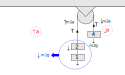
\includegraphics[width=0.8\textwidth]{carrucole.2}
\end{figure}

Sul peso $4$ agiscono queste forze:

\begin{enumerate}
\item[$m_2g$] la forza di gravità
\item[$T$] la tensione della corda
\item[$m_2a$] la forza di inerzia dell'oggetto
\end{enumerate}

La somma delle forze deve essere uguale all'accelerazione risultante.

Il senso delle forze lo conosciamo, quindi:

\end{minipage}

\begin{equation}
m_2g-T=m_2a
\end{equation}

\begin{equation}
\Rightarrow
T=m_2g-m_2a
\end{equation}

L'accelerazione $a$ l'abbiamo calcolata prima: $ a=\frac{g}{7}$

\begin{equation}
\Rightarrow
T=4*10-4*(\frac{10}{7})=34.28571428571428571429
\end{equation}

\begin{minipage}{\textwidth}
\item \textbf{Find the tension in the string connected to the l-kilogram block}

Le forze che agiscono sul peso da 1 kg (chiamiamolo $m$) sono :

\setcounter{equation}{0}
\begin{enumerate}
\item[$mg$] la forza di gravità
\item[$T$] la tensione della corda (l'incognita)
\item[$ma$] la forza di inerzia dell'oggetto
\end{enumerate}

Come prima, la somma delle forze deve essree uguale all'accelerazione risultante.

\begin{equation}
mg -T = -ma
\end{equation}

(stavolta $ma$ è negativa perché va nella direzione opposta a prima)

\begin{equation}
T=mg +ma=1*10+1*\frac{10}{7}= 11.42857142857142857142
\end{equation}

\end{minipage}
\end{enumerate}

\subsubsection{Carrucola e forza di Archimede}

\begin{figure}[h]
\centering
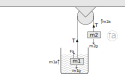
\includegraphics[width=0.8\textwidth]{carrucole.3.pdf}
\end{figure}

Calcolare l'accelerazione $a$ e la tensione della fune sapendo che :

\begin{enumerate}
\item $m1$ è uguale ad 1 kg
\item $m2$ è uguale ad 3 kg
% \item 
\item $m1$ è immerso in un liquido che da origine ad una Forza di Archimede ($Fa$) pari a 1 Newton.
\end{enumerate}
